In this chapter, we discuss how the system is tested both on module level and integration level. We discuss our \emph{performance metrics} and show the results of the system both \emph{quantitatively} and \emph{qualitatively}. We, also, show how our system performs compared to the baselines. Finally, we include the complexity analysis of our system for both time and memory.

\subsection{Testing Setup}

The testing environment of the whole system is basically targeting $4$ main properties :
\begin{enumerate}
    \item The quality of the output face images compared to the real human face images.
    \item The ability of the system to capture the included facial features in the input description and how they actually map to the output.
    \item The smooth and consistent mapping between the edits, imposed on the input description, and the changes of the output face image.
    \item The Independence (\emph{disentanglement}) between the different facial features.
\end{enumerate}

We create our testing strategy to assess these $4$ properties on the output face images. Also, we compare our results against the following baselines :

\begin{itemize}
    \item \texttt{StyleGAN2} \cite{karras2020analyzing} : We compare our results with the original \emph{StyleGAN2} to check the output quality.
    \item \texttt{Faces à la Carte} \cite{wang2020faces} : This is the only previous research work that attempted \emph{Text-to-Face Generation}.
    \item \texttt{Image2StyleGAN} \cite{abdal2019image2stylegan} : Our feature directions extraction methodology is inspired by this work, which is based on the first version of \emph{StyleGAN}.
\end{itemize}

\subsection{Testing Plan and Strategy}

To assess the $4$ previously-mentioned properties, multiple metrics are used, which are listed as follows :
\begin{enumerate}
    \item \textbf{Fréchet Inception Distance} (\emph{FID}) \cite{heusel2018gans} : This metric is an improvement over the traditional \emph{inception score} to be able to measure the similarities between a set of real and synthetic images. Basically, \emph{inception score} measures the ability of \texttt{Inception V3} network \cite{szegedy2014going} to classify a synthetic image into $1000$ classes. However, \emph{FID} measures the distance between synthetic and real images. This is done by extracting $2048D$ feature vector from each image using the \texttt{Inception V3} network and then calculating the \emph{Fréchet} distance using :
    \begin{equation}
        d^2 = ||\textbf{u}_{1} - \textbf{u}_{2}||^2 + Trace(\textbf{C}_{1} + \textbf{C}_{2} - 2 * \sqrt{\textbf{C}_{1} * \textbf{C}_{2}})
    \end{equation}
    Where $\textbf{u}$ is the feature-wise mean vector and $\textbf{C}$ is the covariance matrix of the feature vector.
    
    \item \textbf{Learned Perceptual Image Patch Similarity} (\emph{LPIPS}) \cite{zhang2018unreasonable} : This metric measures the smoothness of the mapping between the latent space edits and the output image changes. This metric takes as an input, two synthetic images. It uses a pretrained neural network to project them to a latent space. Then, it calculates the difference between the two latent vectors, along with the perceptual distance between the two images. Finally, it uses the two distances to calculate the final score. This metric is used in \texttt{StyleGAN2} paper to assess the \emph{perceptual path length}.
    
    \item \textbf{Edit Consistency Score} : We use this metric to ensure that the final facial attributes values are consistent with the input values after the \emph{latent manipulation} process. This metric is simply calculated by projecting the final latent vector over all feature directions and compare it to the input values.
    
    \item \textbf{Directions Disentanglement Score} : The disentanglement between feature directions are assessed by using the \emph{angles} between each pairs of directions. Angles of values $85$ to $95$ degrees usually indicates low entanglement.
\end{enumerate}

\subsubsection{Module Testing}

\paragraph{Speech Recognition}

\paragraph{Text Processing}

\paragraph{Code Generation}
To test the quality of the generated feature directions that are used for \emph{code generation}. We use two methods, which are \textbf{directions disentanglement scores} and \textbf{visual result} of moving along directions.

Table \ref{tab:angles} shows the angles between the directions of a subset of features. Remember that angles in range $85$ to $95$ degrees indicate low entanglement. Consequently, we can infer that the number, provided by the table, are reasonable. For example, the angle between \emph{gray hair} and \emph{age} directions is $79.6$ degrees, because old people normally have gray hair. Also, men are \emph{not} likely to wear makeup, so the angle between \emph{makeup} and \emph{gender} directions is $107.7$ degrees, same for \emph{beard} with men.

Moreover, figure \ref{fig:dir_results} shows the \emph{visual results} of moving along some feature directions. We use these results to qualitatively measure the accuracy of the extracted feature directions.

\begin{table}[ht]
\centering
\begin{tabular}[t]{| c | c | c | c | c |}
\hline
\textbf{Angles} & Age & Gender & Beard & Gray Hair \\
\hline
Age & 0.0 & 92.4 & 85.8 & 79.6 \\
\hline
Gender & 92.4 & 0.0 & 80.0 & 88.6 \\
\hline
Makeup & 88.0 & 107.7 & 100.5 & 94.5 \\
\hline
Hair Length & 89.7 & 95.9 & 90.6 & 96.6 \\
\hline
\end{tabular}
\caption{Angles between different feature directions using a subset of the considered facial features (closer to $90$ degrees is better).}
\label{tab:angles}
\end{table}

\begin{figure}[H]
    \centering
    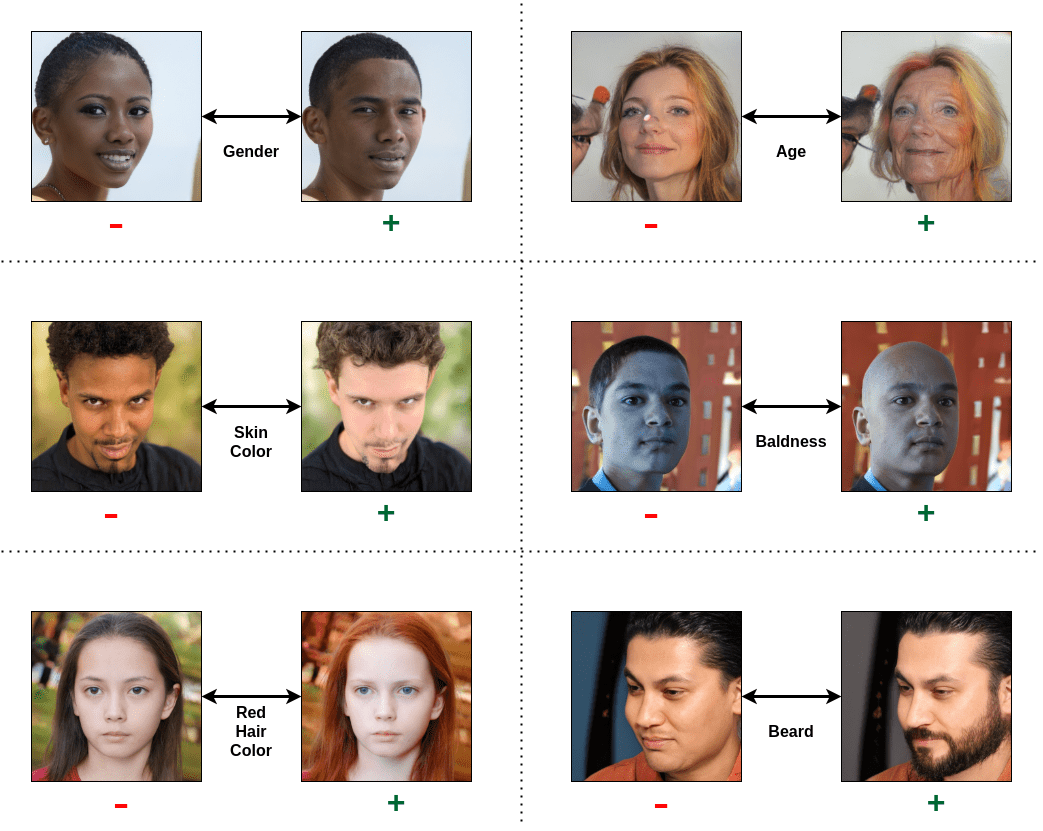
\includegraphics[width=\textwidth]{images/directions-results.png}
    \caption{The results of moving along some extracted feature directions.}
    \label{fig:dir_results}
\end{figure}

\paragraph{Code-to-Face Translation}
This module is basically tested using integration with \textbf{code generation}, which is shown in the \textbf{integration} test. However, we perform testing on this module separately using \textbf{edit consistency score} of the facial attributes values of the output image and the input values. 

As figure \ref{fig:edit_cons} shows, the system can convert a random vector (\emph{on the left}) to the final latent vector (\emph{on the right}) driven by the input values (\emph{on top}). Also, we can see the consistency between the required values and the values corresponding to the generated face.

Also, table \ref{tab:lpips} shows the relation between \emph{LPIPS} score (between the intial and output images) and the number of directions, navigated during face generation. We can see that the score increases, as the number of navigated directions increases. This is mainly because the output face image is far from the initial face image. However, we can see that some \emph{anomalies} can occur, like the case of the input text \emph{"Woman with lipstick and rosy cheeks"}, which navigates along only $3$ directions, but gives a high \emph{LPIPS} score.

\begin{figure}[H]
    \centering
    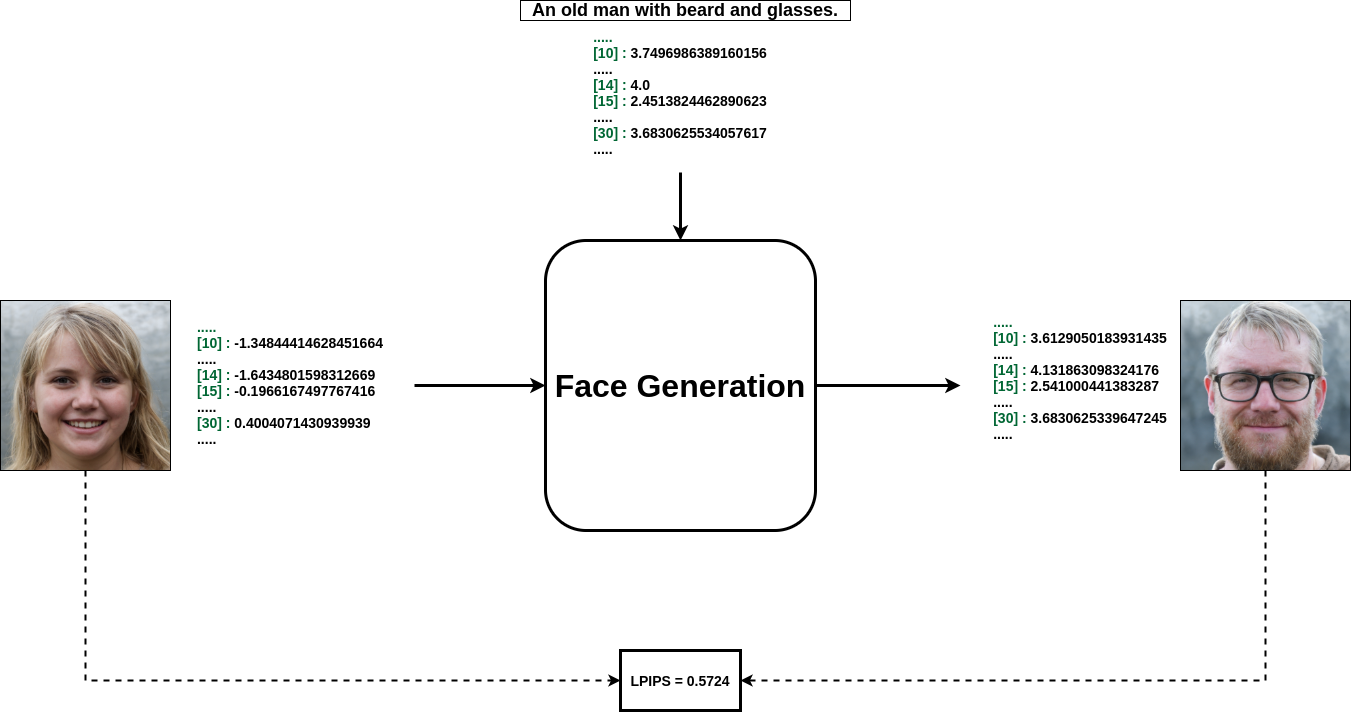
\includegraphics[width=\textwidth]{images/edit-consistency.png}
    \caption{An example of the consistency in reaching the required facial attributes starting from initial random vector.}
    \label{fig:edit_cons}
\end{figure}

\begin{table}[ht]
\centering
\begin{tabular}[t]{| c | c | c |}
\hline
Input Text & Number of Navigated Directions & LPIPS \\
\hline
Female with chubby face & 2 & 0.3905 \\
\hline
Woman with long wavy hair & 3 & 0.4412 \\
\hline
Old black man with glasses & 4 & 0.5023 \\ 
\hline
Woman with lipstick and rosy cheeks & 3 & 0.5107 \\
\hline
Young black man with long hair and beard  & 5 & 0.5733 \\
\hline
Old man with chubby face and glasses & 4 & 0.4905 \\
\hline
\end{tabular}
\caption{LPIPS values against the number of navigated directions for sample text (lower is better).}
\label{tab:lpips}
\end{table}

\paragraph{Face Refinement}
Since, we adapt \texttt{StyleGAN2} for the refinement process, so this module testing is almost the same as \textbf{code-to-face generation} module. However, we focus more on the visuals of the \emph{sequential navigation}, along with the new features related to the face morphology. Figure \ref{fig:nav_res} shows the results of sequential navigation given an original synthetic face image. We tried to maintain the independence of sequential direction navigation as much as possible to keep the results visually acceptable. For example, in the first row, we convert from a \emph{"young man with hear and no beard"} into an \emph{"old bald man with beard"} by sequential navigation using \emph{age}, \emph{beard} and \emph{baldness} directions. This yields much better visual results than many recent \emph{attribute-editing GANs}.

\begin{figure}[H]
    \centering
    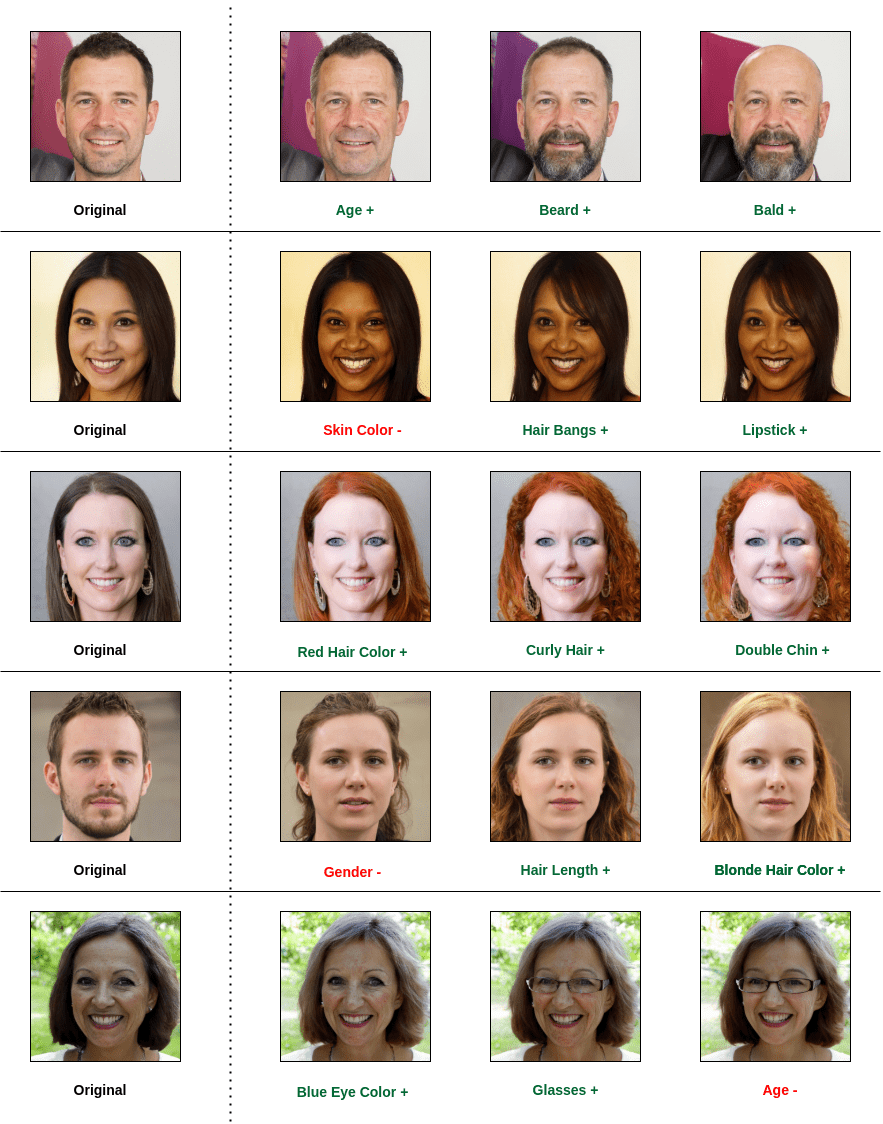
\includegraphics[width=\textwidth]{images/sequential-nav.png}
    \caption{The results of sequential navigation along certain feature directions.}
    \label{fig:nav_res}
\end{figure}

\paragraph{Multiple Head Poses Generation}

\paragraph{Web Application}

\subsubsection{Integration Testing}
The integration of the whole system into a web application is tested qualitatively and quantitatively. In this section, we show the visual results of our system in an \emph{end-to-end} manner. However, we show the quantitative metrics in the comparison with previous work. 

Figures \ref{fig:correct_1} and \ref{fig:correct_2} show correct results of \textbf{face generation} in an \emph{end-to-end} manner using our final \emph{web application}, which contains our complete pipeline. We can see that the results samples are of high accuracy and fidelity. However, of course, the system is \emph{not} $100\%$ accurate. From our extensive testing to the system, we notice $4 types$ of failures, described visually in figure \ref{fig:incorrect}. These failures are listed as follows :
\begin{enumerate}
    \item Failures due to \textbf{contradicting facial features}. As in the \emph{top-left} image, as \emph{rosy cheeks} are very hard to capture with \emph{black skin color}.
    \item Failures due to \textbf{excessive navigation on directions}. As in the \emph{top-right} image, which is very unclear and of low quality with many visual artifacts.
    \item Failures due to \textbf{random initialization}. As in the \emph{bottom-left} image, where sometimes bad initial latent vector can cause the output to be visually inconsistent with many visual artifacts.
    \item Failures due to \textbf{sequential latent manipulation}. As in the \emph{bottom-right} image, where navigation on one direction (\emph{wavy hair}) cancel the navigation on another direction (\emph{short hair}).
\end{enumerate}

\begin{figure}[H]
    \centering
    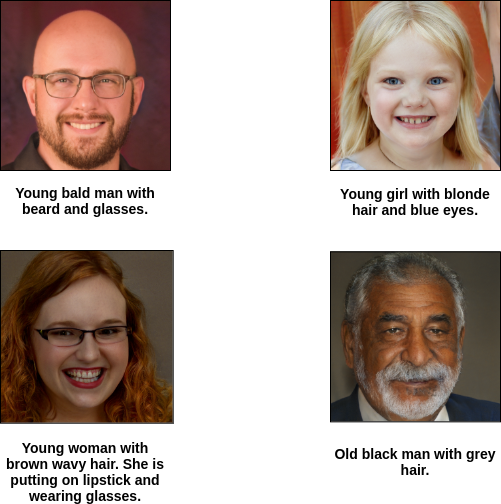
\includegraphics[width=0.8\textwidth]{images/correct-results_1.png}
    \caption{Samples of correctly generated face portrait from textual description.}
    \label{fig:correct_1}
\end{figure}

\begin{figure}[H]
    \centering
    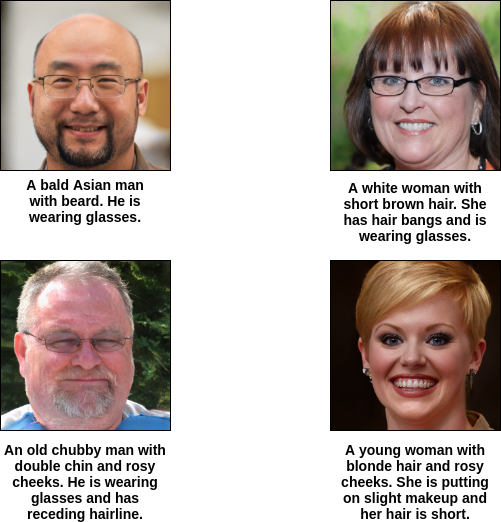
\includegraphics[width=0.8\textwidth]{images/correct-results_2.png}
    \caption{Samples of correctly generated face portrait from textual description.}
    \label{fig:correct_2}
\end{figure}

\begin{figure}[H]
    \centering
    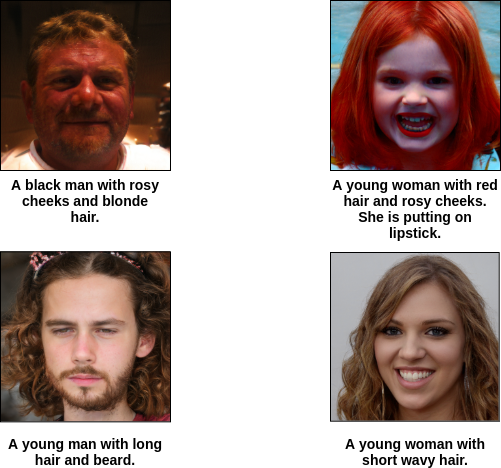
\includegraphics[width=0.8\textwidth]{images/incorrect-results.png}
    \caption{Samples of incorrectly generated face portrait from textual description.}
    \label{fig:incorrect}
\end{figure}

\subsection{Testing Schedule}
Our testing process is scheduled as follows :
\begin{itemize}
    \item First, we conducted the initial testing on the $3$ core modules, while being iteratively designed, until they converged to decent results.
    \item We, then, did the integration testing on these modules separately.
    \item After so, the rest of the system modules were designed and tested separately.
    \item Finally, the whole system was integrated into a single web application and complete testing of the whole system functionalities was conducted.
\end{itemize}

\subsection{Comparative Results to Previous Work}
As mentioned before, we compare our results quantitatively with $3$ baselines, using \textbf{FID score}, \textbf{average LPIPS} and \textbf{execution time}.

Table \ref{tab:fid} and plot \ref{fig:fid} show the comparison of our system to \texttt{StyleGAN2} and \texttt{Image2StyleGAN}. We couldn't include \texttt{Faces à la Carte} in this comparison, as the authors didn't include it in the paper. Also, we couldn't replicate their work, as they didn't provide any specific details about the implementation. We can see that as the number of test images increases, the overall quality of the images increases (\emph{FID} score decreases). Our system performs better than \texttt{Image2StyleGAN}, but worse than the original \texttt{StyleGAN2}, because it is just image generation from random vector with no \emph{latent manipulation} (fewer artifacts).

\begin{table}[ht]
\centering
\begin{tabular}[t]{| c | c | c | c |}
\hline
Test Size & StyleGAN2 & Image2StyleGAN & Our System \\
\hline
50 & 129.15 & 179.58 & 151.58 \\
\hline
100 & 104.29 & 150.54 & 132.54 \\
\hline
200 & 95.25 & 136.45 & 114.45 \\
\hline
300 & 92.44 & 134.04 & 113.04 \\
\hline
400 & 86.37 & 121.59 & 100.59 \\
\hline
500 & 80.09 & 119.02 & 99.02 \\
\hline
\end{tabular}
\caption{FID scores comparison on different number of test images (lower is better).}
\label{tab:fid}
\end{table}

\begin{figure}[H]
    \centering
    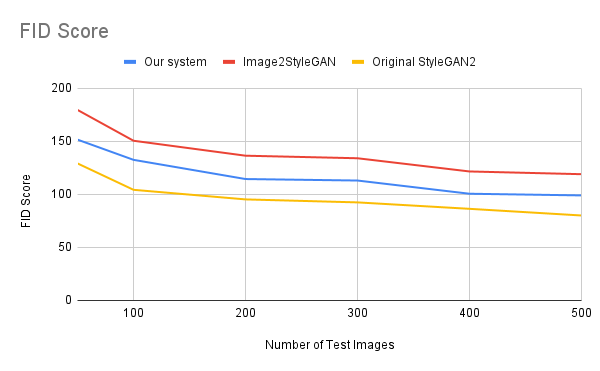
\includegraphics[width=0.8\textwidth]{images/fid_score.png}
    \caption{Plot of FID score of different pipelines against different number of test images (lower is better).}
    \label{fig:fid}
\end{figure}

Next, we compare our system with \texttt{Faces à la Carte} using the only metric, the authors provided, which \emph{LPIPS}. We can see from table \ref{tab:lpips_comp} that our system yields lower overall \emph{LPIPS}, which is better. However, we have higher error margin than \texttt{Faces à la Carte}.

\begin{table}[ht]
\centering
\begin{tabular}[t]{| c | c |}
\hline
Our System & Faces à la Carte \\
\hline
\hline
0.595±0.008 & 0.634±0.005 \\
\hline
\end{tabular}
\caption{LPIPS comparison with Faces à la Carte (lower is better).}
\label{tab:lpips_comp}
\end{table}

Finally, table \ref{tab:exec_time} shows the execution time of different core stages of our system. We can see that the overall \emph{text-to-face generation} process takes only about $0.2$ seconds. However, the web application can take from $1$ second up to multiple seconds to generate a face portrait (from any description) depending on the \emph{connectivity} with the server. Meanwhile, our \emph{multiple head poses generation} module takes around $5$ seconds.

\begin{table}[ht]
\centering
\begin{tabular}[t]{| c | c | c |}
\hline
Text Processing & Latent Manipulation & Face Generation \\
\hline
\hline
0.048 & 0.11 & 0.024 \\
\hline
\end{tabular}
\caption{The execution time of different stages of the core of our system (measured in seconds).}
\label{tab:exec_time}
\end{table}
